\begin{figure*}[t]
    \centering
    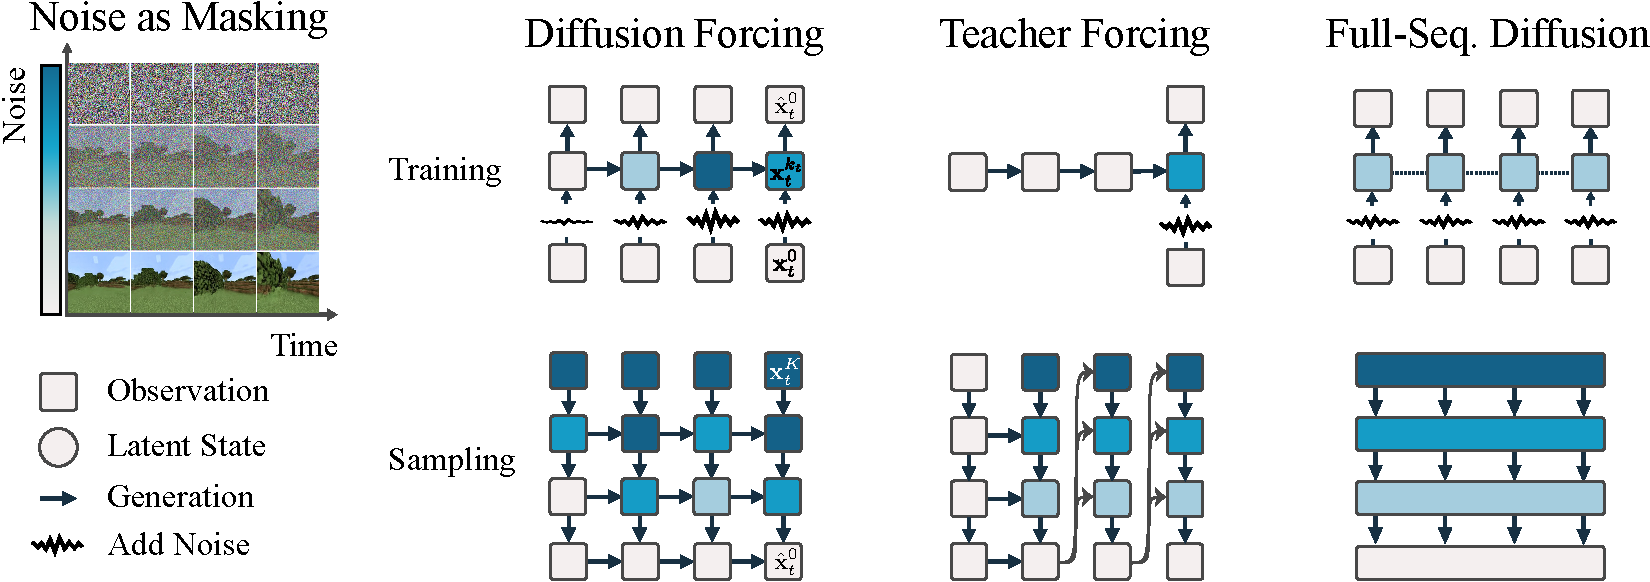
\includegraphics[width=\linewidth]{figures/pdf/Overview_best_guess.pdf}
    \caption{\textbf{Method Overview.} 
    Diffusion Forcing trains causal sequence neural networks (such as an RNN or a masked transformer) to denoise flexible-length sequences where each frame of the sequence can have a \emph{different} noise level.
    In contrast, next-token prediction models, common in language modeling, are trained to predict a single next token from a \emph{ground-truth} sequence (teacher forcing~\cite{teacher_forcing}), and full-sequence diffusion, common in video generation, train non-causal architectures to denoise all frames in a sequence at once with the \emph{same} noise level.
    \algo{} thus \emph{interleaves} the time axis of the sequence and the noise axis of diffusion, unifying strengths of both alternatives and enabling completely new capabilities (see Secs.~\ref{sec:zigzag_example},\ref{sec:method_decision_making}).
    }
    \label{fig:method}
    \vspace{-5pt}
\end{figure*}
